\documentclass[a4paper,10pt]{article}
\usepackage[ngerman]{babel}
\usepackage[utf8]{inputenc}
\usepackage[a4paper,vmargin={20mm,20mm},hmargin={20mm,10mm}]{geometry}
\usepackage[T1]{fontenc}

\usepackage{tocloft, multicol} 
\usepackage{amsmath, amsfonts, amssymb} 
\usepackage{booktabs} 
\usepackage{bm}  
\usepackage{caption}
\usepackage{subcaption}
\usepackage{enumitem}
\usepackage{graphicx} 
\usepackage{listings}
\usepackage{mathtools}
\usepackage[dvipsnames]{xcolor}
\usepackage{wrapfig,lipsum,threeparttable}
\usepackage{footmisc, fixfoot}



\DeclareFixedFootnote{\fnrefa}{ P. T. Boggs and J. E. Rogers, “Orthogonal Distance Regression,” in “Statistical analysis of measurement error models and applications: proceedings of the AMS-IMS-SIAM joint summer research conference held June 10-16, 1989,” Contemporary Mathematics, vol. 112, pg. 186, 1990. }
\DeclareFixedFootnote{\fnrefb}{ Dr. J.Wagner - Physikalisches Anfängerpraktikum - V. 1.1 Stand 1/2018, Versuch 232}


\lstset{literate=%
    {Ö}{{\"O}}1
    {Ä}{{\"A}}1
    {Ü}{{\"U}}1
    {ß}{{\ss}}1
    {ü}{{\"u}}1
    {ä}{{\"a}}1
    {ö}{{\"o}}1
    {~}{{\textasciitilde}}1
}
\lstset{%
backgroundcolor=\color{gray!32},
basicstyle=\ttfamily\footnotesize,
numbers=left,numberstyle=\scriptsize,
frame=single,
breaklines=true,
}

\usepackage[wby]{callouts}
\title{WS19/20, PAP2.1, Versuch 232:\\ Michelson-Interferometer}
\date{Versuchsdurchführung: \\19. November, 2019}
\author{Praktikanten:\\Gerasimov, V., Großmann, J. \& Trautmann, G.\\\\ Betreuer:\\ Wachs, D.}


\begin{document}
\maketitle

\newpage

\tableofcontents

\addtocontents{toc}{~\hfill\textbf{Seite}\par}


\section{Einführung}\boldmath
In diesem Versuch wollen wir unter Berücksichtigung von statistischen Fehlern mit Hilfe eines Michelson-Interferometer verschiedene Messungen durchführen:
\begin{itemize}
\item Die Wellenlänge von einem grünen Laser messen und mit dessen Herstellerangaben vergleichen
\item Den Brechungsindex von Luft für Normalbedingungen  bestimmen und und ihn auch mit den Literaturwerten vergleichen.
\item Die Kohärenzlänge einer Leuchtdiode messen.
\end{itemize}
Dafür verwenden wir die Eigenschaften von Interferenzen gleicher Dicke und Interferenzen gleicher Neigung.
\section{Versuchsaufbau, Literaturwerte \& Vorbereitung}
\begin{itemize}
\item Michelson-Interferometer
\item grüner Laser mit Herstellerangaben der Wellenlänge \(\lambda = (532\pm1) nm\)
\item Leuchtdiode
\item Küvette mit Vakuumpumpe
\item Oszilloskop
\item \( n_{0, Literatur} =1.00028(1)\) als Literaturwert für den Brechungsindex von Luft unter Normalbedingungen
\end{itemize}
\section{Messung der Wellenlänge}
\subsection[Durchführung]{Durchführung\fnrefb}

Wir verstellen den festen Spiegel so, dass wir etwa 2 bis 3 Interferenzringe auf dem Detektor beobachten. Die Öffnung der Irisblende am Detektor wird auf einen Durchmesser von etwa 1 mm eingestellt. Wir schalten das Oszilloskop ein. An Kanal 1 ist direkt das Detektorsignal angeschlossen. Dieses Signal wird zusätzlich auf den Eingang eines Diskriminators gegeben. Die Elektronik bewirkt, dass das Signal nochmals verstärkt wird und in ein Rechtecksignal umgewandelt wird (Abb.\ref{fig:pic1}).\\

\begin{wrapfigure}{r}{0.5\textwidth}
  \centering
  \begin{annotate}{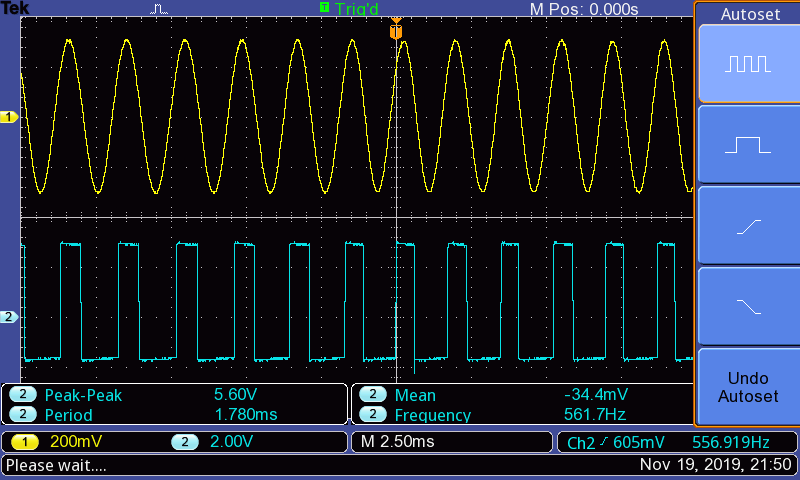
\includegraphics[width=0.5\textwidth]{pic1.png}}{1}
  \end{annotate}
    \caption{Messung der Signale mit einem Oszilloskop}
 \label{fig:pic1}
\end{wrapfigure} 
Jeder Impuls entspricht einem Interferenzmaximum. Die Maxima werden mit dem integrierten Zähler gezählt. Bei der Messung der Wellenlänge ist es wichtig, dass tatsächlich jeder Interferenzstreifen detektiert und gezählt wird. Wir verfahren dazu mit dem Wipptaster der Motorsteuerung den beweglichen Spiegel und beobachten dabei das Oszilloskopbild. Bei jedem Maximum des Sinussignals muss der Diskriminator einen Rechteckpuls ausgeben. Falls dies nicht der Fall ist, kann man folgendes optimieren:
\begin{itemize}
\item Variierung des Durchmessers der Irisblende am Detektor
\item Verstärkung des Detektors (Drehschalter am Detektorgehäuse auf \(60\: dB\) bzw. \(70\: dB\) stellen).
\item Verstärkung des Diskriminators.
\end{itemize}

Die Irisblende sollte nicht zu groß eingestellt werden, sonst mitteln wir über das Interferenzmuster. In der Regel reicht es aus die Verstärkung am Diskriminator zu optimieren. Die Verstärkung sollte aber auch nicht zu groß gewählt werden, sonst wird der Aufbau zu empfindlich und anfällig gegen kleinste
Erschütterungen. Wir machen uns mit der Messuhr vertraut.\\\\
Ein Teilstrich entspricht \(1\: {\mu m}\),\\ eine
volle Zeigerumdrehung  \(0.2\:mm= 200\: {\mu m}\). \\

\unboldmath
\begin{wrapfigure}{r}{0.6\textwidth}
\centering
\captionof{table}{Messung der Wellenlänge}
\begin{threeparttable}
\begin{tabular}{crrr}
\toprule
Messung & Startposition & Endposition & Anzahl der Impulse \\
\(Nr\)&\boldmath\(s_a\) \unboldmath\([mm]\)&\boldmath\(s_e\) \unboldmath\([mm]\)&\boldmath\(m\) \unboldmath\([1]\)\\
\midrule
\(1\)&\(1.000\pm0.009\)&\(3.957\pm0.009\)&\(11092\pm2\)\\
\(2\)&\(3.957\pm0.009\)&\(3.957\pm0.009\)&\(11092\pm2\)\\
\(3\)&\(1.000\pm0.009\)&\(3.957\pm0.009\)&\(11092\pm2\)\\
\(4\)&\(3.957\pm0.009\)&\(3.957\pm0.009\)&\(11092\pm2\)\\
\(5\)&\(1.000\pm0.009\)&\(3.958\pm0.009\)&\(11092\pm2\)\\
  \bottomrule
 \end{tabular}
\begin{tablenotes}
\raggedright
\item[1]sowohl \boldmath\(\Delta s_a\) als auch \(\Delta s_e \) wurdem dem bei der Messuhr ausliegenden Datenblatt entnommen\unboldmath
\item[2] \boldmath\(\Delta m \) grob abgeschätzt\unboldmath
\end{tablenotes}
\end{threeparttable}

\label{tab:Tab1}
\end{wrapfigure}
\boldmath
Wir fahren den Spiegel in Richtung Messuhr
und stellen die Position auf einen Startwert \(s_a\). Beim Einnehmen
der Startposition darf nicht die Verfahrrichtung des Motors nicht geändert werden. Wir notieren bei jedeme Messdurchgang den Startwert \(s_a\). Ab jetzt sind
alle Erschütterungen zu vermeiden. Wir drücken die Resettaste am Zähler und starten den Motor indem wir den rechten oberen Knopf am Motorcontroller
vorsichtig drucken. Der Spiegel bewegt sich nun ca. 3 mm und die dabei durchlaufenden Interferenzmaxima werden vom Zähler registriert. Sobald
der Spiegel angehalten hat notieren wir sofort die gemessenen Impulse. Danach notieren wir auch die Endposition \(s_e\) der Messuhr.
Diese Messung ist insgesamt 5 Mal mit jeweils anderen Werten für \(s_0\) durchzuführen. Da die Messuhr maximal 5 mm aufnehmen kann, muss die Startposition kleiner als 2 mm sein. Für die Wellenlänge \(\lambda\) gilt dann
\begin{equation} \label{eq:lambda}
	\lambda = 2 \frac{|s_e - s_a |}{m}
\end{equation} 
wobei \(m\) die gezählten Impulse sind. Die Genauigkeit der Messuhr \(\Delta s\) können wir
aus dem ausliegenden Datenblatt entnehmen und zu den Messwerten notieren.
\subsection{Messergebnisse}
Messdaten wurden dem Versuchsprotokoll (19. Novemberr, 2019) entnommen und in Tabelle \ref{tab:Tab1} übertragen.
\subsection{Kurvenanpassung mit Python}
\subsubsection{Source Code \& Input}
Wir können \(\lambda\) nach \eqref{eq:lambda} berechnen:
\begin{equation} \tag{\ref{eq:lambda}}
	\lambda = 2 \frac{|s_e - s_a |}{m}
\end{equation}
\begin{equation} \label{eq:Deltalambda}
	\Delta \lambda = \lambda \sqrt{\frac{{\left(\Delta s_a\right)}^2+{\left(\Delta s_e\right)}^2}{\left(s_a - s_e\right)^2}+\left(\frac{\Delta m}{m}\right)^2}
\end{equation}
Wir gehen davon aus, dass die Wellenlänge  konstanmt ist.
Daher ist unser funktionales Modell für die Ausgleichungsrechnung wie folgt:
\begin{equation} \label{eq:Fit1}
	\boxed{\lambda = konst.}
\end{equation} 
So sieht unsere Python-Implementierung aus:\\

Header:
\begin{lstlisting}
%matplotlib inline
import matplotlib.pyplot as plt
import numpy as np
from scipy.optimize import curve_fit
from scipy.signal import hilbert
from scipy.stats import norm
from scipy.stats import chi2
from decimal import Decimal
import csv

def format_e(n):
    a = '%e' % Decimal(n)
    return a.split('e')[0].rstrip('0').rstrip('.')+'e'+a.split('e')[1]

def format_plt(n):
    a = '%e' % Decimal(n)
    return r'${'+a.split('e')[0].rstrip('0').rstrip('.')+'}}$'+r'${*10^{'+a.split('e')[1]+'}}$'
    
def gaussian(x, y, mu, sig):
    return norm.pdf(x, mu, sig)*y
    
\end{lstlisting}

Messwerte aus Tabelle \ref{tab:Tab1} in SI Einheiten:
\begin{lstlisting}

s_a = np.array([1.000,3.957,1.000,3.957,1.000]) *1e-3
Fehler_s_a = np.array([0.009,0.009,0.009,0.009,0.009]) *1e-3

s_e = np.array([3.957,1.000,3.957,1.000,3.958]) *1e-3
Fehler_s_e = np.array([0.009,0.009,0.009,0.009,0.009]) *1e-3

m = np.array([11092,11121,11121,11122,11122]) 
Fehler_m = np.array([2,2,2,2,2])

\end{lstlisting}

Berechnung von \(\lambda\) und \(\Delta \lambda\) nach \eqref{eq:lambda} bzw. \eqref{eq:Deltalambda}:\begin{lstlisting}
lamda = 2*np.abs(s_e-s_a)/m
Fehler_lamda = lamda*np.sqrt((np.sqrt(Fehler_s_a**2+Fehler_s_e**2)/(s_a-s_e))**2+(Fehler_m/m)**2)

\end{lstlisting} 

Nummerierung (um es später darstellen zu können): \begin{lstlisting}
n = np.linspace(1,lamda.size,lamda.size)
Fehler_n = 1e-12

\end{lstlisting} 

Fitfunktion \eqref{eq:Fit1} wird deklariert:\begin{lstlisting}
from scipy import odr

def fit_func(p, x):
    (c) = p
    return x*0+c

model = odr.Model(fit_func)

\end{lstlisting}

darzustellende Daten werden übergeben:\begin{lstlisting}
x = n
y = lamda
delta_x = Fehler_n
delta_y = Fehler_lamda

\end{lstlisting}

Startparameter für Ausgleichungsrechnung werden gesetzt, sodass Lösung konvergiert:\begin{lstlisting}
para0 = [0]

data = odr.RealData(x, y, sx=delta_x, sy=delta_y)
odr = odr.ODR(data, model, beta0=para0 )
out = odr.run()

\end{lstlisting}

Endgültige Ausgleichungsparameter und ihre Kovarianzmatrix werden ausgelesen:\begin{lstlisting}
popt = out.beta
perr = out.sd_beta

\end{lstlisting}

Angabe welche Sigma-Umgebung der Fitfunktion im Diagramm dargestellt werden soll:\begin{lstlisting}
nstd = 1 

popt_top = popt+nstd*perr
popt_bot = popt-nstd*perr

\end{lstlisting}

Plot-Umgebung wird angegeben:\begin{lstlisting}
x_fit = np.linspace(min(x)-(max(x)-min(x))/10, max(x)+3+(max(x)-min(x))/10, 1000)
fit = fit_func(popt, x_fit)
fit_top = fit_func(popt_top, x_fit)
fit_bot = fit_func(popt_bot, x_fit)

\end{lstlisting}

Diagramm (Abb.\ref{fig:Fig1}) wird erstellt:\begin{lstlisting}
y_scale = 1e9
fig, ax = plt.subplots(1, figsize=[6.4 * 1.5, 4.8 * 1.5])
plt.ticklabel_format(axis='both', style='sci', scilimits=(0,3), useMathText=True)
plt.title('Messung der Wellenlänge')
plt.errorbar(x, y*y_scale, yerr=delta_y*y_scale, lw=2, ecolor='k', fmt='none', capsize=8, capthick=2, label='Messdaten')
plt.plot(x_fit, fit*y_scale, 'C3--', lw=2, label='Fit')
plt.plot(x_fit, fit*0+532, 'C0--', lw=2, label='Herstellerangaben')
ax.fill_between(x_fit, fit_top*y_scale, fit_bot*y_scale, color='C3', alpha=.25, label=str(nstd)+'$\sigma$-Umgebung Messung')
ax.fill_between(x_fit, fit_bot*0+532+1, fit_bot*0+532-1, color='C0', alpha=.25, label='1$\sigma$-Umgebung Herstellerangabe')
plt.xlabel('Messung Nr.')
plt.ylabel('Wellenlänge $\lambda$ [nm]')
plt.legend(loc='best')

fig.savefig('figures/232_Fig1.pdf', format='pdf', bbox_inches='tight')

\end{lstlisting}

Der Chi-Quadrat-Test wird durchgeführt unter Berücksichtigung von \( \Delta t\) und \(\Delta \omega\). D.h.~es wird jeweils der senkrechte/orthogonale Abstand der Messwerte zur Fitfunktion (Abb.\ref{fig:chi}) berechnet und normiert\fnrefa.
 Die Summe der normierten Abstandsquadrate, der \unboldmath\( \chi^{2}\)-Wert, wird  reduziert.\boldmath

\begin{figure}[htb]
  \centering
  \begin{annotate}{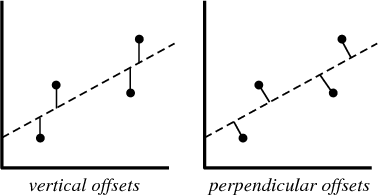
\includegraphics[width=0.5\textwidth]{chi.png}}{1}
  \end{annotate}
\caption[Abstände von Messdaten zur Fitfunktion]{Abstände von Messdaten zur Fitfunktion\footnotemark}
\label{fig:chi}
\end{figure}
\footnotetext{http://mathworld.wolfram.com/LeastSquaresFitting.html}

\begin{lstlisting}
dof = x.size-popt.size
chisquare = np.sum(((fit_func(popt, x)-y)**2)/(delta_y**2+((fit_func(popt, x+delta_x)-fit_func(popt, x-delta_x))/2)**2))
chisquare_red = chisquare/dof
prob = round(1-chi2.cdf(chisquare,dof),2)*100

\end{lstlisting}

Auslesen der Messergebnisse:\begin{lstlisting}
lamda_mean = popt[0]
Fehler_lamda_mean = perr[0]

\end{lstlisting}

Ausgabe der Messergebnisse wird erstellt:\begin{lstlisting}
print('Wellenlänge:')
print('lambda [m] =', format_e(lamda_mean), ' +- ', format_e(Fehler_lamda_mean))
print('Chi-Quadrat =', chisquare)
print('Freiheitsgrade =', dof)
print('Chi-Quadrat reduziert =', chisquare_red)
print('Wahrscheinlichkeit ein größeres oder gleiches Chi-Quadrat zu erhalten =', prob, '%')

\end{lstlisting}

\subsubsection{Output}
\begin{lstlisting}
Wellenlänge:
lambda [m] = 5.320805e-07  +-  2.750607e-10
Chi-Quadrat = 0.28801824173344576
Freiheitsgrade = 4
Chi-Quadrat reduziert = 0.07200456043336144
Wahrscheinlichkeit ein größeres oder gleiches Chi-Quadrat zu erhalten = 99.0 %

\end{lstlisting}
Wir erfahren also sofort, dass
\begin{align*}
\lambda&=532.08(28)\:nm
\end{align*}
und als Ergebnis auf unseren Anpassungstest:
\[\chi^{2}_{red}=7.2\times10^{-2}\]
Die Wahrscheinlichkeit ein größeres oder gleiches Chi-Quadrat zu erhalten ist
 \[P\approx  99.0 \%\]
und wir erhalten das Diagramm in Abb.\ref{fig:Fig1}.

\begin{figure}[htb]
  \centering
  \begin{annotate}{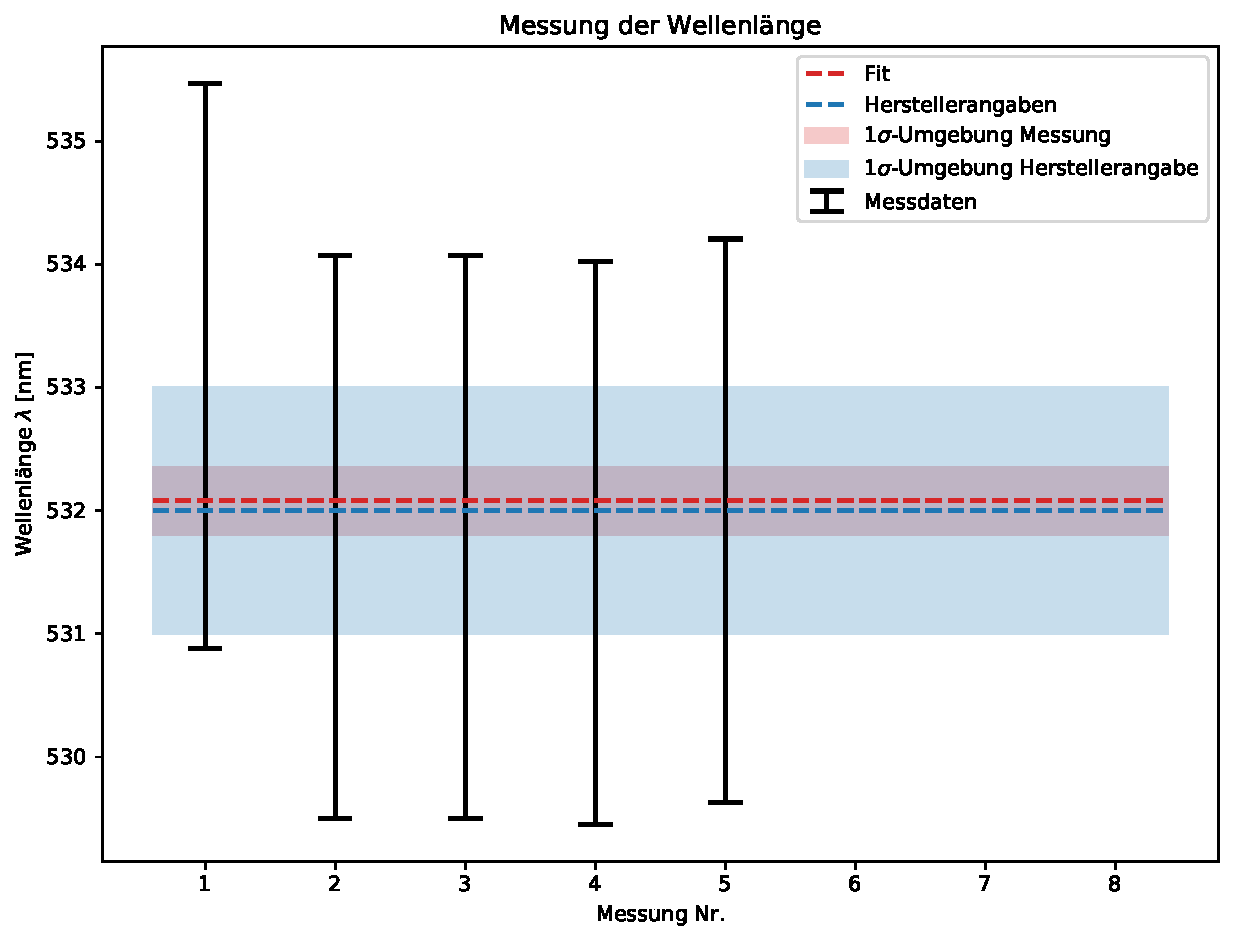
\includegraphics[width=0.8\textwidth]{232_Fig1.pdf}}{1}
  \end{annotate}
\caption{}
\label{fig:Fig1}
\end{figure}
\pagebreak
\subsection{Auswertung}
Der Messwert und die Herstellerangabe
\begin{align*}
\lambda&=532.08(28)\:nm\\
\lambda_{Hersteller}&=532.0(10)\:nm
\end{align*}
liegen jeweils in der 1-Sigma-Umgebung von einander. D.h. sie unterscheiden sich nicht signifikant von einander. Der relativ geringe Chi-Quadrat-Wert
\(\chi^{2}_{red}=7.2\times10^{-2}\) ist wahrscheinlich einer sehr konservativen Wahl unserer Fehler geschuldet. Der deutlich größere Fehler laut Herstellerangabe ist wahrscheinlich ein willkürlich aufgerundeter Wert auf ganze Nanometer. Es ist zu erwarten das der Hersteller in der Lage wäre
die Wellenlänge \(\lambda \) genauer zu messen als wir und gegebenenfalls theoretisch zu bestätigen.
\pagebreak
\section{Messung des Brechungsindex von Luft}
\subsection[Durchführung]{Durchführung\fnrefb}
\unboldmath
\begin{wrapfigure}{r}{0.55\textwidth}
\centering
\captionof{table}{des Brechungsindex von Luft}
\begin{threeparttable}
\begin{tabular}{crr}
\toprule
Messreihe & Anzahl der verstrichenen Ringe & Druck \\
\( Nr\)&\boldmath\(m\) \unboldmath\( [1] \)&\boldmath\( p'\) \unboldmath\( [Torr]\) \\
\midrule
\(1\)&\(0\pm2\)&\(-743\pm5\)\\
\(''\)&\(10\pm2\)&\(-670\pm5\)\\
\(''\)&\(15\pm2\)&\(-595\pm5\)\\
\(''\)&\(20\pm2\)&\(-515\pm5\)\\
\(''\)&\(25\pm2\)&\(-440\pm5\)\\
\(''\)&\(30\pm2\)&\(-365\pm5\)\\
\(''\)&\(35\pm2\)&\(-290\pm5\)\\
\(''\)&\(40\pm2\)&\(-200\pm5\)\\
\(''\)&\(45\pm2\)&\(-135\pm5\)\\
\(''\)&\(50\pm2\)&\(-55\pm5\)\\
\(''\)&\(55\pm2\)&\(0\pm5\)\\
\midrule
\(2\)&\(0\pm2\)&\(-744\pm5\)\\
\(''\)&\(10\pm2\)&\(-665\pm5\)\\
\(''\)&\(15\pm2\)&\(-590\pm5\)\\
\(''\)&\(20\pm2\)&\(-525\pm5\)\\
\(''\)&\(25\pm2\)&\(-440\pm5\)\\
\(''\)&\(30\pm2\)&\(-360\pm5\)\\
\(''\)&\(35\pm2\)&\(-290,\pm5\)\\
\(''\)&\(40\pm2\)&\(-215\pm5\)\\
\(''\)&\(45\pm2\)&\(-140\pm5\)\\
\(''\)&\(50\pm2\)&\(-60\pm5\)\\
\midrule
\(3\)&\(0\pm2\)&\(-745\pm5\)\\
\(''\)&\(10\pm2\)&\(-670\pm5\)\\
\(''\)&\(15\pm2\)&\(-595\pm5\)\\
\(''\)&\(20\pm2\)&\(-515\pm5\)\\
\(''\)&\(25\pm2\)&\(-440\pm5\)\\
\(''\)&\(30\pm2\)&\(-365\pm5\)\\
\(''\)&\(35\pm2\)&\(-290\pm5\)\\
\(''\)&\(40\pm2\)&\(-213\pm5\)\\
\(''\)&\(45\pm2\)&\(-155\pm5\)\\
\(''\)&\(50\pm2\)&\(-60\pm5\)\\
 \bottomrule
 \end{tabular}
\begin{tablenotes}
\raggedright
\item[1] \boldmath\(\Delta p\)  wurden als  0,6\% vom Skalenendwert (800 Torr) abgeschätzt\fnrefb\unboldmath
\item[2] \boldmath\(\Delta m \) grob abgeschätzt\unboldmath
\end{tablenotes}
\end{threeparttable}
\label{tab:Tab2}
\end{wrapfigure}
\boldmath
Als Lichtquelle wird weiterhin der grüne Laser benutzt. Den Schirm wird vor dem Detektor platziert und vor dem festen Spiegel auf Position 3 die Küvette. Der feste Spiegel wird so eingestellt, dass auf dem Schirm 2-3 Interferenzringe zu sehen sind. Wir schließen  das Nadelventil indem wir den Einstellknopf ganz nach rechts drehen, schalten die Vakuumpumpe ein und öffnen den Absperrhebel solange, bis sich der Druck in der Küvette nicht mehr ändert. Danach können wir
den Absperrhebel wieder schließen und die Pumpe ausschalten. Mittels des Nadelventils lässt man in die evakuierte Gaszelle langsam Luft einströmen. Dabei
quellen aus dem Zentrum neue Interferenzringe hervor. Wir lesen nach je 5 Interferenzringen den Druck \(p'\) am Manometer ab, wobei \(p=p'+b\) Wir führen die Messung dreimal durch und notieren zusätzlich die Zimmertemperatur \(T\).\\

Wir berechnen den Brechungsindex von Luft für Normalbedingungen. Ist \(n_0\) der
Brechungsindex bei Normalbedingungen, dann gilt:
\begin{equation}
	 \frac{n_0 -1}{n\left(p\right)-1} = \frac{p_0 T}{p T_0}
\end{equation} 
Mit Hilfe von Gleichung \eqref{eq:gl38}
\begin{equation} \label{eq:gl38}
	 n \left( \lambda, R, b\right)-1 = m \frac{\lambda}{2a} b
\end{equation}
wobei \(b\) den äußeren Luftdruck und \(a\) das Innenmaß der Küvette darstellt. Daraus folgt dann:
\begin{equation}\label{eq:gl41}
	 \left({n_0 -1}\right)= \left({n -1}\right)\frac{p_0}{p}\frac{T}{T_0}=\frac{\lambda}{2a}\frac{m}{p}\frac{p_0 T}{T_0}
\end{equation} 
Die Normalbedingungen sind festgelegt und \(a\) ist angegeben\fnrefb als:
\begin{align*}
T_0&=273.15\:K\\
p_0&=1013.25\:hPa\\
a&=50.00(5)\:mm
\end{align*}

\subsection{Messergebnisse}
Messdaten wurden dem Versuchsprotokoll (19. Novemberr, 2019) entnommen und in Tabelle \ref{tab:Tab2} übertragen.\\
Die Raumtemperatur ist \(T=23.8(2)\:^{\circ}C\) mit dem Fehler \(\Delta T\) abgeschätzt aus der Inhomogenität des Anzeigewerts am Thermometer während der Versuchszeit.
\subsection{Kurvenanpassung mit Python, Schritt 1}
\subsubsection{Source Code \& Input}
Wir gehen davon aus, dass die Präzessionsdauer proportional zur Eigenkreisfrequenz zunimmt.
Daher ist unser funktionales Modell für die Ausgleichungsrechnung wie folgt:
\begin{equation} \label{eq:Fit2}
	\boxed{p' = mS + konst.}
\end{equation} 

So sieht die Fortführung unserer Python-Implementierung aus:\\

Messwerte aus Tabelle \ref{tab:Tab2} in SI Einheiten (wobei \(m\) für die einzelnen Messreihen relative verschoben wurden, um sie besseer darstellen zu können):
\begin{lstlisting}
m_1 = np.array([0,10,15,20,25,30,35,40,45,50,55]) 
Fehler_m_1 = np.array([2,2,2,2,2,2,2,2,2,2,2])

m_2 = np.array([0,10,15,20,25,30,35,40,45,50]) +10 
Fehler_m_2 = np.array([2,2,2,2,2,2,2,2,2,2])

m_3 = np.array([0,10,15,20,25,30,35,40,45,50]) +20 
Fehler_m_3 = np.array([2,2,2,2,2,2,2,2,2,2])

p_1 = np.array([-743,-670,-595,-515,-440,-365,-290,-200,-135,-55,0]) *(101325/760)
Fehler_p_1 = np.array([5,5,5,5,5,5,5,5,5,5,5]) *(101325/760)

p_2 = np.array([-744,-665,-590,-525,-440,-360,-290,-215,-140,-60]) *(101325/760)
Fehler_p_2 = np.array([5,5,5,5,5,5,5,5,5,5]) *(101325/760)

p_3 = np.array([-745,-670,-595,-515,-440,-365,-290,-213,-155,-60]) *(101325/760)
Fehler_p_3 = np.array([5,5,5,5,5,5,5,5,5,5]) *(101325/760)
\end{lstlisting}

Fitfunktion \eqref{eq:Fit2} wird deklariert:\begin{lstlisting}
from scipy import odr

def fit_func(p, x):
    (s, c) = p 
    return s*x+c

model = odr.Model(fit_func)

\end{lstlisting}

darzustellende Daten werden übergeben:\begin{lstlisting}
x_1 = p_1
y_1 = m_1
delta_x_1 = Fehler_p_1
delta_y_1 = Fehler_m_1

x_2 = p_2
y_2 = m_2
delta_x_2 = Fehler_p_2
delta_y_2 = Fehler_m_2

x_3 = p_3
y_3 = m_3
delta_x_3 = Fehler_p_3
delta_y_3 = Fehler_m_3

\end{lstlisting}

Startparameter für Ausgleichungsrechnung werden gesetzt, sodass Lösung konvergiert:\begin{lstlisting}
para0 = [0, 0]

data_1 = odr.RealData(x_1, y_1, sx=delta_x_1, sy=delta_y_1)
odr_1 = odr.ODR(data_1, model, beta0=para0 )
out_1 = odr_1.run()

data_2 = odr.RealData(x_2, y_2, sx=delta_x_2, sy=delta_y_2)
odr_2 = odr.ODR(data_2, model, beta0=para0 )
out_2 = odr_2.run()

data_3 = odr.RealData(x_3, y_3, sx=delta_x_3, sy=delta_y_3)
odr_3 = odr.ODR(data_3, model, beta0=para0 )
out_3 = odr_3.run()

\end{lstlisting}

Endgültige Ausgleichungsparameter und ihre Kovarianzmatrix werden ausgelesen:\begin{lstlisting}
popt_1 = out_1.beta
perr_1 = out_1.sd_beta

popt_2 = out_2.beta
perr_2 = out_2.sd_beta

popt_3 = out_3.beta
perr_3 = out_3.sd_beta

\end{lstlisting}

Angabe welche Sigma-Umgebung der Fitfunktion im Diagramm dargestellt werden soll:\begin{lstlisting}
nstd = 1 

popt_top_1 = popt_1+nstd*perr_1
popt_bot_1 = popt_1-nstd*perr_1

popt_top_2 = popt_2+nstd*perr_2
popt_bot_2 = popt_2-nstd*perr_2

popt_top_3 = popt_3+nstd*perr_3
popt_bot_3 = popt_3-nstd*perr_3

\end{lstlisting}

Plot-Umgebung wird angegeben:\begin{lstlisting}
x_fit = np.linspace(min(min(x_1),min(x_2),min(x_3))*1.1, min(min(x_1),min(x_2),min(x_3))*(-0.1), 1000)

fit_1 = fit_func(popt_1, x_fit)
fit_top_1 = fit_func(popt_top_1, x_fit)
fit_bot_1 = fit_func(popt_bot_1, x_fit)

fit_2 = fit_func(popt_2, x_fit)
fit_top_2 = fit_func(popt_top_2, x_fit)
fit_bot_2 = fit_func(popt_bot_2, x_fit)

fit_3 = fit_func(popt_3, x_fit)
fit_top_3 = fit_func(popt_top_3, x_fit)
fit_bot_3 = fit_func(popt_bot_3, x_fit)

\end{lstlisting}

Diagramm (Abb.\ref{fig:Fig2}) wird erstellt:\begin{lstlisting}
fig, ax = plt.subplots(1, figsize=[6.4 *1.5, 4.8])
plt.ticklabel_format(axis='both', style='sci', scilimits=(0,3), useMathText=True)
plt.errorbar(x_1, y_1, yerr=delta_y_1, xerr=delta_x_1, lw=1, ecolor='k', fmt='none', capsize=1, label='Messreihe 1')
plt.errorbar(x_2, y_2, yerr=delta_y_2, xerr=delta_x_2, lw=1, ecolor='k', fmt='none', capsize=1, label='Messreihe 2')
plt.errorbar(x_3, y_3, yerr=delta_y_3, xerr=delta_x_3, lw=1, ecolor='k', fmt='none', capsize=1, label='Messreihe 3')
plt.title('Messung der Steigung $S_i$ = $\Delta m_i / p$ pro Messreihe')
plt.grid(True)
plt.xlabel('Druck $p+p_0$ [Pa]')
plt.ylabel('$m$')
plt.plot(x_fit, fit_1, color='C0', lw=1, label='Fit  1')
plt.plot(x_fit, fit_2, color='C2', lw=1, label='Fit  2')
plt.plot(x_fit, fit_3, color='C3', lw=1, label='Fit  3')
ax.fill_between(x_fit, fit_top_1, fit_bot_1, color='C0', alpha=.25, label=str(nstd)+r'$\sigma$'+'-Umgebung 1')
ax.fill_between(x_fit, fit_top_2, fit_bot_2, color='C2', alpha=.25, label=str(nstd)+r'$\sigma$'+'-Umgebung 2')
ax.fill_between(x_fit, fit_top_3, fit_bot_3, color='C3', alpha=.25, label=str(nstd)+r'$\sigma$'+'-Umgebung 3')
box = ax.get_position()
ax.set_position([box.x0, box.y0, box.width * 0.8, box.height])
ax.legend(loc='center left', bbox_to_anchor=(1, 0.5))

plt.savefig('figures/232_Fig2.pdf', format='pdf', bbox_inches='tight')

\end{lstlisting}

Der Chi-Quadrat-Test wird durchgeführt unter Berücksichtigung von \(\Delta \omega_F\) und \(\Delta T_P\). D.h.~es wird jeweils der senkrechte/orthogonale Abstand der Messwerte zur Fitfunktion (Abb.\ref{fig:chi}) berechnet und normiert\fnrefa.

\begin{lstlisting}
dof_1 = x_1.size-popt.size
chisquare_1 = out_1.sum_square
chisquare_red_1 = chisquare_1/dof_1
prob_1 = round(1-chi2.cdf(chisquare_1,dof_1),2)*100

dof_2 = x_2.size-popt.size
chisquare_2 = out_2.sum_square
chisquare_red_2 = chisquare_2/dof_2
prob_2 = round(1-chi2.cdf(chisquare_2,dof_2),2)*100

dof_3 = x_3.size-popt.size
chisquare_3 = out_3.sum_square
chisquare_red_3 = chisquare_3/dof_3
prob_3 = round(1-chi2.cdf(chisquare_3,dof_3),2)*100

\end{lstlisting}

Auslesen der Messergebnisse:\begin{lstlisting}
S_1 = popt_1[0]
Fehler_S_1 = perr_1[0]
S_2 = popt_2[0]
Fehler_S_2 = perr_2[0]
S_3 = popt_3[0]
Fehler_S_3 = perr_3[0]

\end{lstlisting}

Ausgabe der Messergebnisse wird erstellt:\begin{lstlisting}
print('Steigungen: ')
print('S_1 [1/Pa] =', format_e(S_1), ' +- ', format_e(Fehler_S_1))
print('Chi-Quadrat =', chisquare_1)
print('Freiheitsgrade =', dof_1)
print('Chi-Quadrat reduziert =', chisquare_red_1)
print('Wahrscheinlichkeit ein größeres oder gleiches Chi-Quadrat zu erhalten =', prob_1, '%')
print('\n')
print('S_2 [1/Pa] =', format_e(S_2), ' +- ', format_e(Fehler_S_2))
print('Chi-Quadrat =', chisquare_2)
print('Freiheitsgrade =', dof_2)
print('Chi-Quadrat reduziert =', chisquare_red_2)
print('Wahrscheinlichkeit ein größeres oder gleiches Chi-Quadrat zu erhalten =', prob_2, '%')
print('\n')
print('S_3 [1/Pa] =', format_e(S_3), ' +- ', format_e(Fehler_S_3))
print('Chi-Quadrat =', chisquare_3)
print('Freiheitsgrade =', dof_3)
print('Chi-Quadrat reduziert =', chisquare_red_3)
print('Wahrscheinlichkeit ein größeres oder gleiches Chi-Quadrat zu erhalten =', prob_3, '%')
\end{lstlisting}
\subsubsection{Output}
\begin{lstlisting}
Steigungen: 
S_1 [1/Pa] = 5.171618e-04  +-  1.381261e-05
Chi-Quadrat = 4.683194878131682
Freiheitsgrade = 10
Chi-Quadrat reduziert = 0.46831948781316823
Wahrscheinlichkeit ein größeres oder gleiches Chi-Quadrat zu erhalten = 91.0 %

S_2 [1/Pa] = 5.224287e-04  +-  1.573934e-05
Chi-Quadrat = 4.0422956700548145
Freiheitsgrade = 9
Chi-Quadrat reduziert = 0.44914396333942386
Wahrscheinlichkeit ein größeres oder gleiches Chi-Quadrat zu erhalten = 91.0 %

S_3 [1/Pa] = 5.248941e-04  +-  1.589543e-05
Chi-Quadrat = 4.082827181272153
Freiheitsgrade = 9
Chi-Quadrat reduziert = 0.45364746458579475
Wahrscheinlichkeit ein größeres oder gleiches Chi-Quadrat zu erhalten = 91.0 %

\end{lstlisting}
Wir erfahren also sofort, dass
\begin{align*}
S_1&=5.17(14)\times10^{-4}\:{Pa}^{-1}\\
S_2&=5.22(16)\times10^{-4}\:{Pa}^{-1}\\
S_3&=5.25(16)\times10^{-4}\:{Pa}^{-1}
\end{align*}
und als Ergebnis auf unseren Anpassungstests:
\begin{align*}
\chi^{2}_{red,1}&=4.7\times10^{-1}\\
\chi^{2}_{red,2}&=4.5\times10^{-1}\\
\chi^{2}_{red,3}&=4.5\times10^{-1}
\end{align*}
Die Wahrscheinlichkeiten ein größeres oder gleiches Chi-Quadrat zu erhalten sind jeweils
\begin{align*}
P_1\approx  91.0 \%\\
P_2\approx  91.0 \%\\
P_3\approx  91.0 \%\\
\end{align*}
(Rechnung mehrmals überprüft. Alle 3 Werte stimmen wirklich auf zwei Stellen überein)\\
und wir erhalten das Diagramm in Abb.\ref{fig:Fig2}.

\begin{figure}[htb]
  \centering
  \begin{annotate}{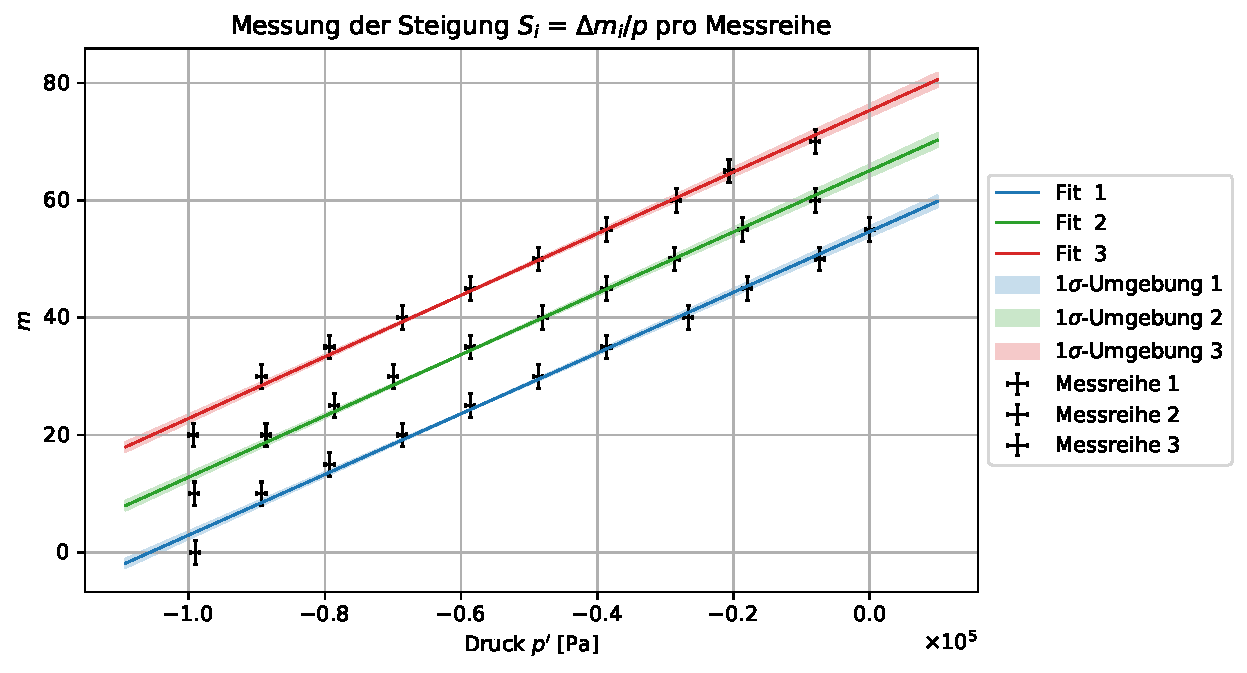
\includegraphics[width=0.8\textwidth]{232_Fig2.pdf}}{1}
  \end{annotate}
\caption{}
\label{fig:Fig2}
\end{figure}
\subsection{Kurvenanpassung mit Python, Schritt 2}
\subsubsection{Source Code \& Input}
Wir gehen davon aus, dass der Brechungsindex konstant ist.
Daher ist unser funktionales Modell für die Ausgleichungsrechnung wie folgt:
\begin{equation} \label{eq:Fit3}
	\boxed{n_0 = konst.}
\end{equation} 
Für diesen Schritt, benutzen wir die Angaben aus "Versuchsaufbau, Literaturwerte \& Vorbereitung" 
\begin{align*}
T_0&=273.15\:K\\
p_0&=1013.25\:hPa\\
a&=50.00(5)\:mm
\end{align*}
unser Ergebnis für \(\lambda\) aus der vorherigen Messung
\begin{align*}
\lambda&=532.08(28)\:nm\\
\end{align*}
und die Messergebnisse aus Schritt 1 um den Brechungsindex nach \eqref{eq:gl41} zu berechnen:
\begin{equation} \label{eq:n_0}
	n_0= 1+\frac{\lambda}{2a}\frac{\Delta m}{p}\frac{p_0 T}{T_0} = 1+ S \frac{\lambda}{2a}\frac{p_0 T}{T_0}
\end{equation} 
\begin{equation} \label{eq:Deltan_0}
	\Delta n_0= \frac{\lambda S p_0 T}{2 a T_0} \sqrt{{\left(\frac{\Delta \lambda}{\lambda}\right)}^2+{\left(\frac{\Delta S}{S}\right)}^2+{\left(\frac{\Delta T}{T}\right)}^2+{\left(\frac{\Delta a}{a}\right)}^2}
\end{equation} 
So sieht die Fortführung unserer Python-Implementierung aus:\\

Messwerte der Steigung S aus Schritt 1 in SI Einheiten:
\begin{lstlisting}
S = np.array([S_1,S_2,S_3])
Fehler_S = np.array([Fehler_S_1,Fehler_S_2,Fehler_S_3])

\end{lstlisting}

Raumtemperatur \( T\) in SI Einheiten:
\begin{lstlisting}
T = 23.8 +273.15
Fehler_T = 0.2

\end{lstlisting}

Normalbedingungen in SI Einheiten:
\begin{lstlisting}
p_0 = 101325
T_0 = 273.15

\end{lstlisting}

Innenmaß der Küvette \( a\) in SI Einheiten:
\begin{lstlisting}
a = 50 *1e-3
Fehler_a = 0.05 *1e-3

\end{lstlisting}

Berechnung des Brechungsindex  \(n_0\) und \(\Delta n_0\) nach \eqref{eq:n_0} bzw. \eqref{eq:Deltan_0}:\begin{lstlisting}
n_0 = 1+lamda_mean*S*p_0*T/(2*a*T_0)
Fehler_n_0 = lamda_mean*S*p_0*T/(2*a*T_0)*np.sqrt((Fehler_lamda_mean/lamda_mean)**2+(Fehler_S/S)**2
                                                       +(Fehler_T/T)**2+(Fehler_a/a)**2)

\end{lstlisting} 

Nummerierung (um es später darstellen zu können): \begin{lstlisting}
N = np.linspace(1,S.size,S.size)
Fehler_N = 1e-12

\end{lstlisting}

Fitfunktion \eqref{eq:Fit3} wird deklariert:\begin{lstlisting}
from scipy import odr

def fit_func(p, x):
    (c) = p # c: Konstante
    return x*0+c

model = odr.Model(fit_func)

\end{lstlisting}

darzustellende Daten werden übergeben:\begin{lstlisting}
x = N
y = n_0
delta_x = Fehler_N
delta_y = Fehler_n_0

\end{lstlisting}

Endgültige Ausgleichungsparameter und ihre Kovarianzmatrix werden ausgelesen:\begin{lstlisting}
para0 = [0]

data = odr.RealData(x, y, sx=delta_x, sy=delta_y)
odr = odr.ODR(data, model, beta0=para0 )
out = odr.run()

\end{lstlisting}

Endgültige Ausgleichungsparameter und ihre Kovarianzmatrix werden ausgelesen:\begin{lstlisting}
popt = out.beta
perr = out.sd_beta

\end{lstlisting}

Angabe welche Sigma-Umgebung der Fitfunktion im Diagramm dargestellt werden soll:\begin{lstlisting}
nstd = 1 # um n-Sigma-Umgebung im Diagramm zu zeichnen

popt_top = popt+nstd*perr
popt_bot = popt-nstd*perr

\end{lstlisting}

Plot-Umgebung wird angegeben:\begin{lstlisting}
x_fit = np.linspace(min(x)-(max(x)-min(x))/10, max(x)+3+(max(x)-min(x))/10, 1000)
fit = fit_func(popt, x_fit)
fit_top = fit_func(popt_top, x_fit)
fit_bot = fit_func(popt_bot, x_fit)

\end{lstlisting}

Diagramm (Abb.\ref{fig:Fig3}) wird erstellt:\begin{lstlisting}
fig, ax = plt.subplots(1, figsize=[6.4 * 1.5, 4.8 * 1.5])
plt.ticklabel_format(axis='both', style='sci', scilimits=(0,3), useMathText=True)
plt.title('Messung des Brechungsindex')
plt.errorbar(x, y, yerr=delta_y, lw=2, ecolor='k', fmt='none', capsize=8, capthick=2, label='Ergebnisse der Messreihen')
plt.plot(x_fit, fit, 'C3--', lw=2, label='Fit')
ax.fill_between(x_fit, fit_top, fit_bot, color='C3', alpha=.25, label=str(nstd)+'$\sigma$-Umgebung Fit')
plt.plot(x_fit, fit*0+1.00028, 'C0--', lw=2, label='Literaturwert')
plt.xlabel('Messreihe Nr.')
plt.ylabel('Brechungsindex $n_0$')
plt.legend(loc='best')

fig.savefig('figures/232_Fig3.pdf', format='pdf', bbox_inches='tight')

#Chi-Quadrat orthogonal
dof = x.size-popt.size
chisquare = np.sum(((fit_func(popt, x)-y)**2)/(delta_y**2+((fit_func(popt, x+delta_x)-fit_func(popt, x-delta_x))/2)**2))
chisquare_red = chisquare/dof
prob = round(1-chi2.cdf(chisquare,dof),2)*100

#Auswertung
n_0_mean = popt[0]
Fehler_n_0_mean = perr[0]

#Ausgabe
print('Brechungsindex:')
print('n_0 =', n_0_mean, ' +- ', format_e(Fehler_n_0_mean))
print('Chi-Quadrat =', chisquare)
print('Freiheitsgrade =', dof)
print('Chi-Quadrat reduziert =', chisquare_red)
print('Wahrscheinlichkeit ein größeres oder gleiches Chi-Quadrat zu erhalten =', prob, '%')

\end{lstlisting}
\subsubsection{Output}
\begin{lstlisting}
Brechungsindex:
n_0 = 1.000305408647939  +-  1.373493e-06
Chi-Quadrat = 0.14506966547849148
Freiheitsgrade = 2
Chi-Quadrat reduziert = 0.07253483273924574
Wahrscheinlichkeit ein größeres oder gleiches Chi-Quadrat zu erhalten = 93.0 %

\end{lstlisting}
Wir erfahren also sofort, dass
\begin{align*}
n_0&=1.0003054(14)
\end{align*}
und als Ergebnis auf unseren Anpassungstest:
\[\chi^{2}_{red}=7.3\times10^{-2}\]
Die Wahrscheinlichkeit ein größeres oder gleiches Chi-Quadrat zu erhalten ist
 \[P\approx  93.0 \%\]
und wir erhalten das Diagramm in Abb.\ref{fig:Fig3}.
\begin{figure}[htb]
  \centering
  \begin{annotate}{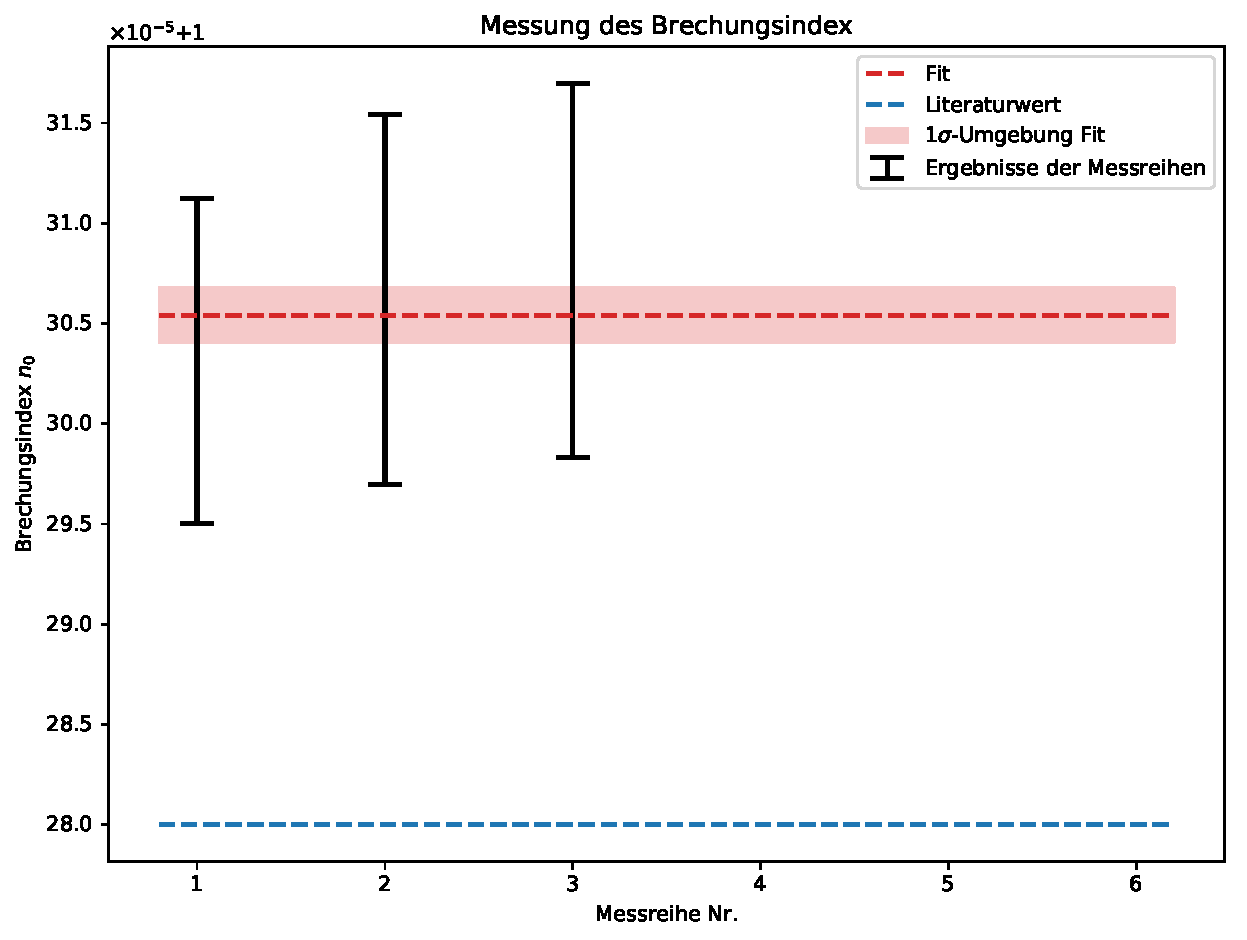
\includegraphics[width=0.8\textwidth]{232_Fig3.pdf}}{1}
  \end{annotate}
\caption{}
\label{fig:Fig3}
\end{figure}

\subsection{Auswertung}
Die gemessenen Wert für \(n_0\) passt zwar Sinn und passen zu unserem theoretischen Modellen \eqref{eq:Fit2} und \eqref{eq:Fit3}, da keine signifikant abweichenden Chi Quadratwerte auftrafen und Wahrscheinlichkeiten ein größeres oder gleiches Chi-Quadrat zu erhalten waren:
\begin{align*}
P_1\approx  91.0 \%\\
P_2\approx  91.0 \%\\
P_3\approx  91.0 \%\\
P\approx  93.0 \%
\end{align*}
Daran lässt sich lässt sich aber vermuten, dass unsere abgeschätzten Messfehler \(\Delta p\) und \(\Delta m\) zu groß waren. Auf signifikante systematische Fehler lassen die Werte aber nicht schließen. Der Vergleich von Messergebnis und Literaturwert lässt dagegen deutlich werden, dass bei uns an irgendeiner Stelle doch systematische Fehler aufgetreten sein müssen:
\begin{align*}
n_0&=1.0003054(14) \\
n_{0, Literatur} &=1.00028(1)
\end{align*}
Da der Literaturwert nur sehr grob angegeben wurde, handelt es sich nur um eine \(2.5\sigma\)-signifikante Differenz.
\[\frac{ n_{0, Literatur}- n_0}{\sqrt{(\Delta  n_{0, Literatur})^2+(\Delta n_0)^2}}= 2.5\]
Damit ist die Wahrscheinlichkeit, dass diese Differenz hauptsächlich statistisch bedingt ist nur \[1-erf{\left({\frac{2.5}{\sqrt{2}}}\right)} \approx 1.2\%\]
Stellen an denen die dafür verantwortlichen statistische Fehler auftreten können, können im Versuchsaufbau aufgetreten sein (z.B. Volumen der Küvette), menschlicher Natur sein (grobes Verzählen, falsche Ablesung der Messwerte) oder physikalische Abhängigkeiten sein, die wir einfach nur vernachlässigt haben (z.B. Luftfeuchtigkeit). Versuch wurde nicht ausführlich genug wiederholt um darüber im Nachhinein eine detaillierte Aussage treffen zu können.

\section{Messung der Kohärenzlänge einer Leuchtdiode}
\subsection[Durchführung]{Durchführung\fnrefb}
Wir entfernen die Küvette aus dem Strahlengang und verfahren den beweglichen Spiegel in den Bereich der Weißlichtposition. Der ungefähre Wert ist auf dem Interferometer angegeben. Man stellt den festen Spiegel so ein, dass wir sehr große Interferenzstrukturen zu sehen sind, d.h. möglichst nur einen Ring. Anstatt des Lasers bauen wir nun die Leuchtdiode ein, entfernen die \(-50\:mm\) Linse vor dem Detektor und richten die Leuchtdiode so aus, dass wir den Schatten des Strahlteilers zentrisch auf dem Detektor sehen. Die Öffnung der Irisblende am Detektor sollte etwa \(1-2\:mm\) sein. Danach stellen wir die Verstärkung des Detektors auf das Maximum ein (\(70\:db\)).\\ 

Da die Kohärenzlänge der Leuchtdiode sehr klein ist, sind Interferenzen nur über einen sehr kleinen Verfahrweg beobachtbar. Um diese mit dem Oszilloskop darzustellen, muss das Oszilloskop im Single-Modus betrieben werden. In diesem Modus \glqq wartet\grqq~das Oszilloskop auf ein Signal einer gewissen Größe, welches wir mit dem Triggerlevel einstellen können. Sobald ein Signal anliegt welches den Level übersteigt, beginnt das Oszilloskop mit der Aufzeichnung und speichert den Signalverlauf. Eine Anleitung zur Einstellung des Single- Modus liegt aus. Wir stellen die y-Ablenkung auf \(50\:mV\) und legen den Triggerlevel gerade etwas über den Rauschpegel, so dass das Oszilloskop im Single- Modus nicht auslöst.\\ \begin{wrapfigure}{r}{0.5\textwidth}
  \centering
  \begin{annotate}{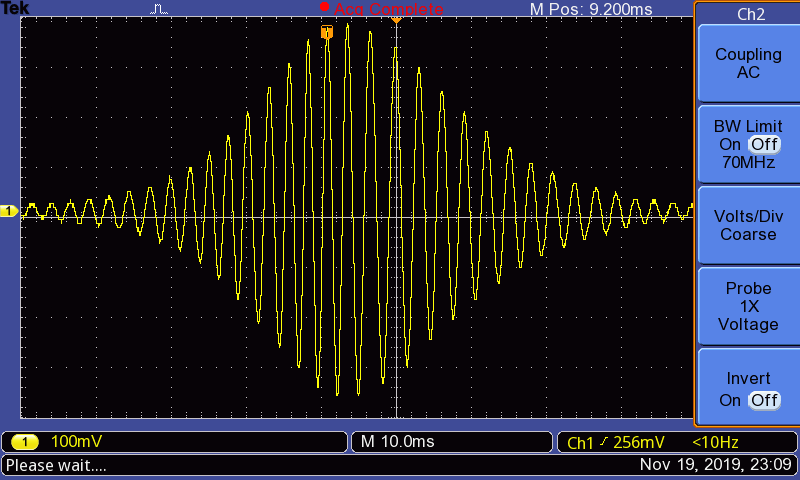
\includegraphics[width=0.5\textwidth]{pic2.png}}{1}
  \end{annotate}
    \caption{Signalverlauf am Oszilloskop zu den  Interferenzstrukturen}
 \label{fig:pic2}
\end{wrapfigure} 
Das Oszilloskop stellen wir scharf und verfahren den beweglichen Spiegel in Richtung Strahlteiler. Dazu den Wippschalter des Motorcontrollers ganz nach oben drucken und halten. Sobald wir auf die Weißlichtposition kommen löst das Oszilloskop aus und speichert das Signal. Dann lassen wir sofort den Wippschalter los und stellen den Schirm vor den Detektor. Den Spiegel sehr langsam fahren wir in die entgegengesetzte Richtung bis Interferenzen sichtbar werden.\\

Danach entfernen wir den Schirm und wiederholen die Messung mit optimierten Oszilloskopeinstellungen. Z.B. entfernen wir eine Umdrehung der Messuhr von der Weißlichtposition und fahren dann mit maximaler Geschwindigkeit zurück durch die Weißlichtposition (Wippschalter ganz durchdrücken). Den Signalverlauf speichern wir auf einen USB- Stick.

\subsection{Messergebnisse}
Messdaten wurden unter der CSV-Datei\\\texttt{data\textbackslash Messung2\textbackslash Messung2\_CH1.csv}\\  (19. Novemberr, 2019) und als BMP-Bild in Abbildung \ref{fig:pic2} gespeichert.\\

\subsection{Auswertung und Darstellung mit Python}
\subsubsection{Source Code \& Input}
Wir drücken \(t\) über den entsprechenden Verfahrensweg \(x\) aus:
\begin{equation} \label{eq:x}
	x = tv
\end{equation} 
Die Fehler der Werte \(\Delta v\), \(\Delta t\) und \(\Delta x\) sehen wir in diesem Versuch als vernachlässigbar klein an.\\
So sieht die Fortführung unserer Python-Implementierung aus:\\

Verfahrensgeschwindigkeit \(v\) in SI Einheiten:
\begin{lstlisting}
v_Verfahren = 0.1 *1e-3


\end{lstlisting}

Messwerte aus CSV-Datei in SI Einheiten:\begin{lstlisting}
t = np.array([])
V = np.array([])
with open('data\Messung2\Messung2_CH1.csv') as csv_file:
    csv_reader = csv.reader(csv_file, delimiter=',')
    for row in csv_reader:
        t = np.append(t,float(row[3]))
        V = np.append(V,float(row[4]))

\end{lstlisting}

Berechnung des Verfahrensweges \(x\) nach \eqref{eq:x}:\begin{lstlisting}
x = t*v_Verfahren

\end{lstlisting}

Signalverarbeitung zur Erzeugung  einer Einhüllenden:\begin{lstlisting}
analytic_signal = hilbert(V)
amplitude_envelope = np.abs(analytic_signal)

\end{lstlisting}

Anpassung der Einhüllenden an eine Normalverteilung  über die Zeit:\begin{lstlisting}
fitParams, fitCovariances = curve_fit(gaussian, t, amplitude_envelope)

\end{lstlisting}

Auslesen der Messergebnisse und Umwandlung der Abhängigkeit von Zeit zur Abhängigkeit vom Weg:\begin{lstlisting}
mu = fitParams[1]*v_Verfahren
sigma = fitParams[2]*v_Verfahren
counts = t.size

\end{lstlisting}

Diagramm (Abb.\ref{fig:Fig4}) wird erstellt:\begin{lstlisting}
fig, ax = plt.subplots(1, figsize=[6.4 *1.5, 4.8])
plt.ticklabel_format(axis='both', style='sci', scilimits=(0,3), useMathText=True)
plt.plot(x, V, lw=1, color='C3', marker='', alpha=.50, label='Signal')
plt.plot(x,gaussian(t,*fitParams),  lw=1, color='C0', label='Normalverteilung:\n'
         +r'${\mu}$'+' = '+str(format_plt(mu))+' m\n'
         +r'${\sigma}$'+' = '+str(format_plt(sigma))+' m\n'
         +r'$FWHM = $'+format_plt(sigma*2.355)+' m')
plt.title('Messung der Kohärenzlänge einer Leuchtdiode')
plt.ylabel('Spannung U [V]')
plt.xlabel('Verfahrensweg x [m]')
plt.grid(True)
plt.legend(loc='best')

fig.savefig('figures/232_Fig4.pdf', format='pdf', bbox_inches='tight')

\end{lstlisting}

Ausgabe der Messergebnisse wird erstellt:\begin{lstlisting}
print('Anzahl der Messungen = ', counts)
print('Normalverteilung:\n'
         +'mu = '+str(format_e(mu))+' m\n'
         +'sigma = '+str(format_e(sigma))+' m\n'
         +'FWHM = '+format_e(sigma*2.355)+' m')
         
\end{lstlisting}
\subsubsection{Output}
\begin{lstlisting}
Anzahl der Messungen =  2500
Normalverteilung:
mu = 3.973149e-07 m
sigma = 1.392349e-06 m
FWHM = 3.278981e-06 m

\end{lstlisting}
Wir erfahren also sofort, dass die Einhüllende des Signalverlaufs, also der räumlichen Interferenzstruktur ungefähr einer Normalverteilung folgt, mit den folgenden Parametern:
\begin{align*}
\mu&= 3.973149\times10^{-7} m\\
\sigma&= 1.392349\times10^{-6} m\\
FWHM&= 3.27898\times10^{-6} m
\end{align*}
und ein Bild der angepassten Normalverteilung und der Interferenzstrukturen in Abbildung \ref{fig:Fig4}.
\begin{figure}[htb]
  \centering
  \begin{annotate}{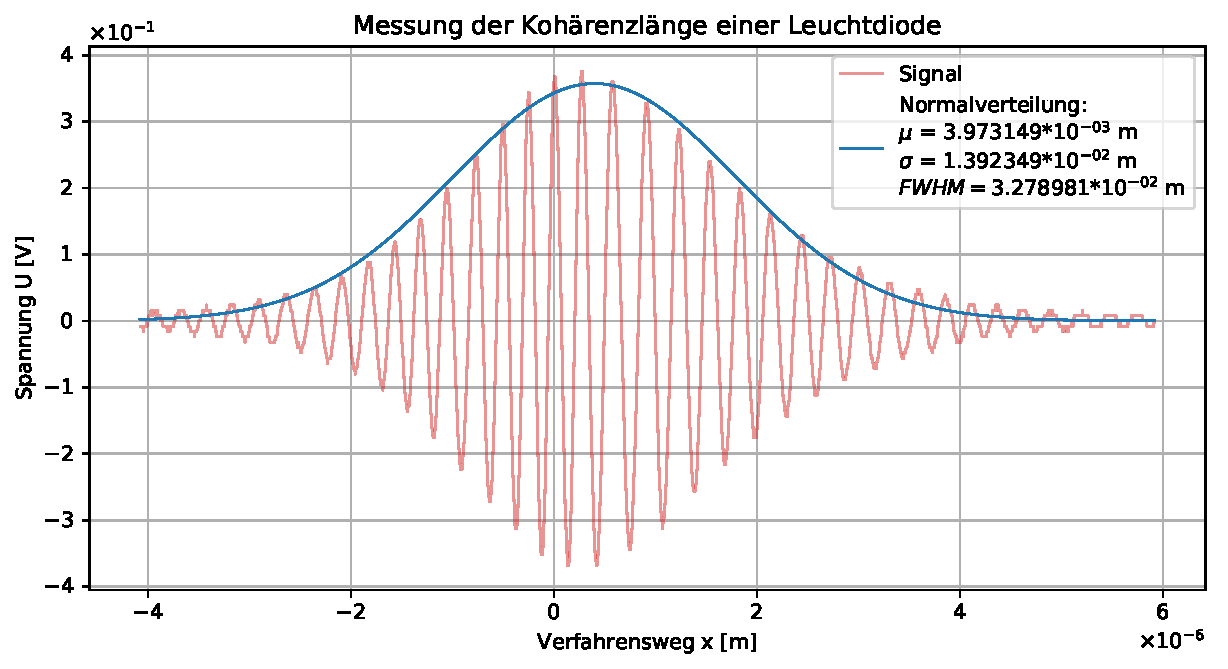
\includegraphics[width=0.8\textwidth]{232_Fig4.pdf}}{1}
  \end{annotate}
\caption{}
\label{fig:Fig4}
\end{figure}
\subsection{Auswertung}
Die Kohärenzlänge \(l_c\) der Leuchtdiode entspricht genau der bestimmten Halbwertsbreite \(FWHM\) (eng. Abkürzung für: Full Width at Half Maximum):
\begin{align*}
l_c = FWHM = 3.27898\:{\mu m}
\end{align*}
Weil wir zuvor uns dazu entschieden haben keine Fehler bei diesem Teilversuch zu betrachten, haben wir auch keinen Fehler \(\Delta l_c\) bestimmt.
\section{Fazit}
\begin{itemize}
\item Die Wellenlänge von einem grünen Laser wurde auf bestimmt und stimmt mit den Herstellerangaben (Differenz kleiner als \(1\sigma\)).
\begin{align*}
\lambda&=532.08(28)\:nm\\
\lambda_{Hersteller}&=532.0(10)\:nm
\end{align*}
\item Der Brechungsindex von Luft für Normalbedingungen wurde bestimmt und und mit den Literaturwerten verglichen. Die Differenz zwischen ihnen beträgt 2.5 Sigma. Unbeachtete systematische Fehler, die signifikant das Ergebnis verändert haben, sind zu vermuten (siehe Auswertung).
\begin{align*}
n_0&=1.0003054(14) \\
n_{0, Literatur} &=1.00028(1)
\end{align*}
\item Die Kohärenzlänge der uns gegebenen Leuchtdiode wurde auf ungefähr \(l_c  = 3.28\:{\mu m}\) bestimmt. Größenordnungsmäßig liegt das unter gewöhnlichem Feinstaub.
\end{itemize}
\unboldmath
\end{document}
